%****************************************************************************%
%* DIET Programmer's Guide - Annexe 1                                       *%
%*                                                                          *%
%*  Author(s):                                                              *%
%*    - Christophe PERA (christophe.pera@ens-lyon.fr)                       *%
%*                                                                          *%
%* $LICENSE$                                                                *%
%****************************************************************************%
%* $Id$
%* $Log$
%* Revision 1.2  2006/03/17 16:42:56  eboix
%*    Cmake is now briefly commented in the programmer's guide. --- Injay2461
%*
%* Revision 1.1  2004/01/09 15:26:53  cpera
%* Add Annexe on Autotools.
%*
%****************************************************************************%


% This is detail description about autotools files
\appendix{Autotools in depth}

%\section{Autotools in depth}
This annexe describes autotools files. All its content is from "The Goat Book"
by Gary V. Vaughan, Ben Elliston, Tom Tromey and Ian Lance Taylor, published 
in October 2000 by New Riders publishing and freely available online at 
http://sources.redhat.com/autobook/autobook/autobook.html.

%\footnote{"GNU autoconf, automake and libtool" from Gary V. Vaughan, Ben Elliston, Tom Tromey and Ian Lance Taylor {\url{http://sources.redhat.com/autobook/autobook/autobook.html}}}

\section{CMake: managing the build process}

\subsection{Introduction}
CMake is used to control the software compilation process using simple platform
and compiler independent configuration files.
Seen from Diet software developer's point of view, the description of
Diet's build process is achieved exclusively by writing simple configuration
files which are placed in each directory (that requires some building action)
of the source hierarchy.
Those configuration files called CMakeLists.txt are used to generate standard
build files (e.g. makefiles on Unix and projects/workspaces in Windows MSVC).
Each CMakeLists.txt consists of one or more commands, where each command
has the form \texttt{COMMAND (args...)} where \texttt{COMMAND} is the name
of the command, and args is a white-space separated list of arguments.
Among the numerous pre-defined commands of CMake the ones defining a target
(something to be build e.g. a library, a binary, a documentation...) are of
particular interest:
\begin{itemize}
\item \texttt{ADD\_LIBRARY( )} adds a library to the list of targets,
\item \texttt{ADD\_EXECUTABLE( )} adds an executable to the list of targets,
      (Note: source code is compiled first, then libraries are built, and
       then executables are created.)
\item \texttt{ADD\_SUBDIRECTORY( )} which enables a directory-based recursive
      description of the CMakeLists.txt hierarchy, although directories are
      not targets,
\item \texttt{ADD\_CUSTOM\_TARGET( )} which adds any specific target required
      by the developper (e.g. the documentation).
\end{itemize}
As for every language, developpers writing CMakeLists.txt configuration
files should resist the temptation of obfuscation. When exceptional
CMake's tricks are required please bear in mind that the \texttt{\#}
character is used to denote a comment line. Comment or perish...

\subsection{Target hierarchy}
The hierarchy of CMakeLists.txt configuration files describes a hierarchy
of target dependencies together with the associated commands that need to be
invoked in order to restore a broken dependency.
But you should not expect the recursive traversal of the target
hierarchy to be related in any way to the CMakeLists.txt's hierarchy
recursive traversal.
Further than that the relative line order of \texttt{ADD\_SUBDIRECTORY( )}
occurences within a single CMakeLists.txt is not significative.
Hence, developpers need to explicitely express all target dependencies 
at the risk of describing an erroneous building process.

\subsection{External package dependency}
Diet makes a heavy usage of external functionalities starting with
compilers (C, C++, Java, TeX, Doxygen), functionalities provided by system
calls or libraries (OmniOrb, BLAS, JXTA, AppleSeeds...).
The dependencies toward those external tools are expressed in so-called
Find modules (and technically realised as CMake MACROs).
Although CMake already provides many such Find modules, some project 
packagers do not yet provide their respective Find module (e.g. OmniOrb).
The directory DIET/Cmake provides all the Find modules required by Diet
and not yet considered as standard by CMake.
When a DIET developper adds an new external dependency (say towards a
library) it is his reponsability to make sure the corresponding 
Find module is available. When this module is not available the
developper must provide one and place it in the DIET/Cmake subdirectory.

\subsection{CMake references and documentation}
Some links worth to mention:
\begin{itemize}
\item \url{http://www.cmake.org/HTML/Documentation.html} for the official
      on-line documentation (including all \texttt{COMMAND} description),
\item \url{http://www.cmake.org/Wiki/CMake} for CMake users Wiki,
\item \url{http://www.cmake.org/HTML/MailingLists.html} for searching
      CMake's very active mailing lists,
\item "Mastering CMake" book (see
      \url{http://www.kitware.com/products/cmakebook.html}).
\end{itemize}

\section{bootstrapping}
Bootstrap.sh is a shell script calling :
\begin{enumerate}
\item{libtoolize}
\item{aclocal}
\item{autoheader}
\item{automake}
\item{autoconf}
\end{enumerate}

\subsection{aclocal}
The aclocal program creates the file `aclocal.m4' by combining stock installed
macros, programer defined macros and the contents of `acinclude.m4' to define all
of the macros required by `configure.in' in a single file. Aclocal was 
created as a fix for some missing functionality in Autoconf. Aclocal is a part of
automake package.

%\begin{figure}[h]
\begin{center}
\includegraphics[scale=.35]{fig/DiagrammeAclocal.eps}
\end{center}
%\label{fig:aclocal}
%\caption{Aclocal files}
%\end{figure}

\subsection{autoheader}
autoheader runs m4 over `configure.in', but with key macros defined differently
than when autoconf is executed, such that suitable cpp definitions are output
to "DIET\_config.h.in". It is a part of autoconf package.

\begin{center}
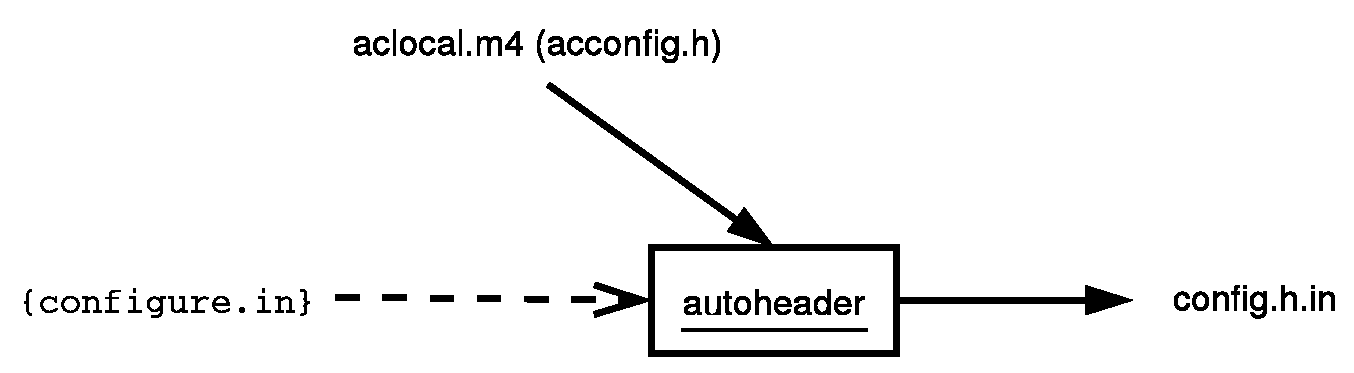
\includegraphics[scale=.35]{fig/DiagrammeAutoheader.ps}
\end{center}

\subsection{Automake and Libtoolize}
Automake\footnote{Automake {\url{http://www.gnu.org/software/automake/automake.html}}} 
will call libtoolize to generate some extra files if the macro 
'AC\_PROG\_LIBTOOL' is used in `configure.in'. If it is not present 
then automake will install `config.guess' and `config.sub' by itself.

libtoolize\footnote{Libtool {\url{http://www.gnu.org/software/libtool/libtool.html}}}
can also be run manually if desired. 
Automake will only run libtoolize automatically if `ltmain.sh' and `ltconfig' 
are missing. In DIET, we choose to call explicitly libtoolize before automake
in bootstrap.sh.

\begin{center}
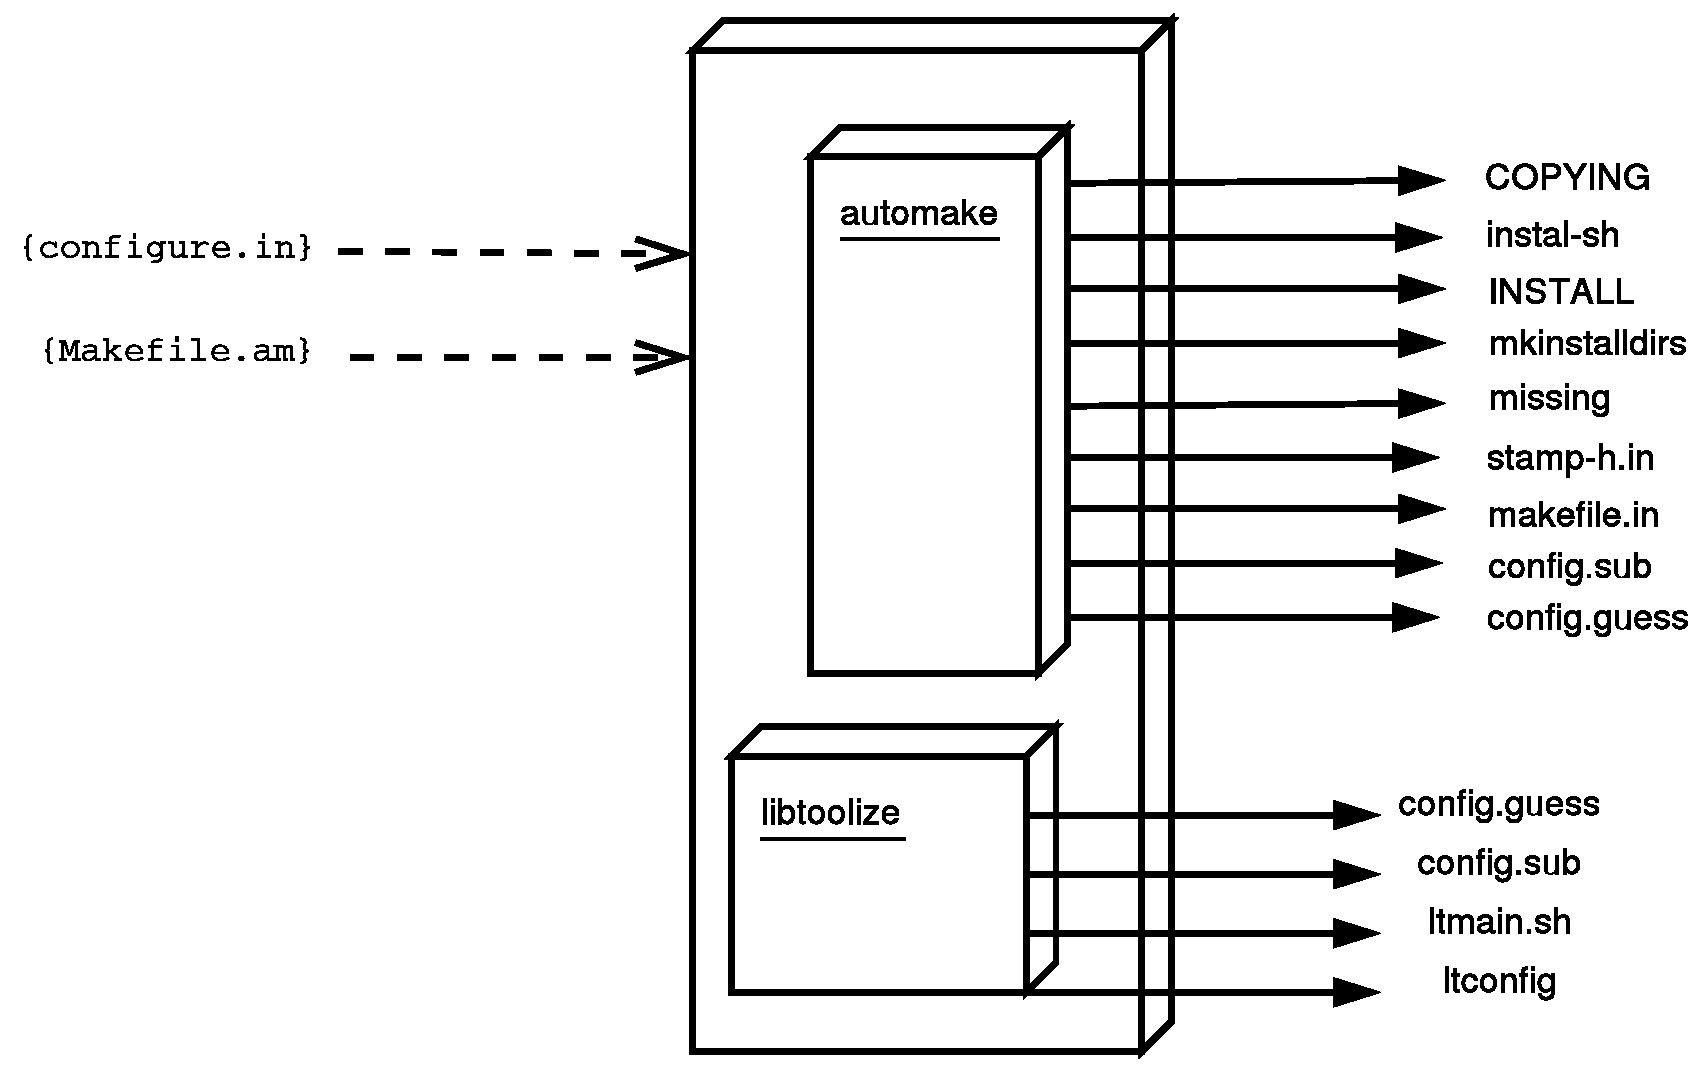
\includegraphics[scale=.35]{fig/DiagrammeAutomakeLibtoolize.ps}
\end{center}

The versions of `config.guess' and `config.sub' installed differ between 
releases of Automake and Libtool, and might be different depending on whether 
libtoolize is used to install them or not. Before releasing your own package 
you should get the latest versions of these files from ftp://ftp.gnu.org/gnu/config,
in case there have been changes since releases of the GNU Autotools.
Currently, DIET is developped with, at least, libtool 1.4.3, automake 1.7.3 and 
autoconf 2.57. Bootstraping and compiling may succeed with others previous autotools version
but it is not garanteed.
%\footnote{Automake {\url{http://www.gnu.org/software/automake/automake.html}}}
%\footnote{Libtool {\url{http://www.gnu.org/software/libtool/libtool.html}}}


\subsection{autoconf}
autoconf\footnote{Autoconf {\url{http://www.gnu.org/software/autoconf/}}} expands the m4 macros in `configure.in', using macro 
definitions from `aclocal.m4', to generate the configure script.
\begin{center}
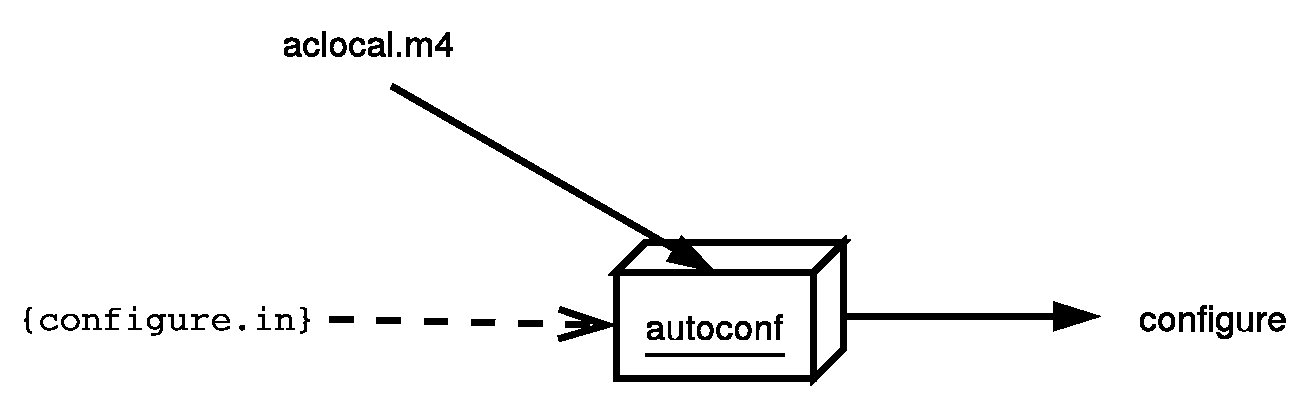
\includegraphics[scale=.35]{fig/DiagrammeAutoconf.ps}
\end{center}
%\footnote{Autoconf {\url{http://www.gnu.org/software/autoconf/}}}

\subsection{configure}
The purpose of the preceding processes was to create the input files necessary
for configure to run correctly. You would ship your project with the generated
script and the files in columns, other input and processes (except 
`config.cache'), but configure is designed to be run by the person installing
your package. Naturally, you will run it too while you develop your project,
but the files it produces are specific to your development machine, and are
not shipped with your package -- the person installing it later will run 
configure and generate output files specific to their own machine.

Running the configure script on the build host executes the various tests 
originally specified by the `configure.in' file, and then creates another script,
`config.status'. This new script generates the `DIET\_config.h' header file from 
`DIET\_config.h.in', and `Makefile's from the named `Makefile.in's. Once 
`config.status' has been created, it can be executed by itself to regenerate
files without rerunning all the tests. Additionally, `AC\_PROG\_LIBTOOL'
was used, so ltconfig is used to generate a libtool script. 

\begin{center}
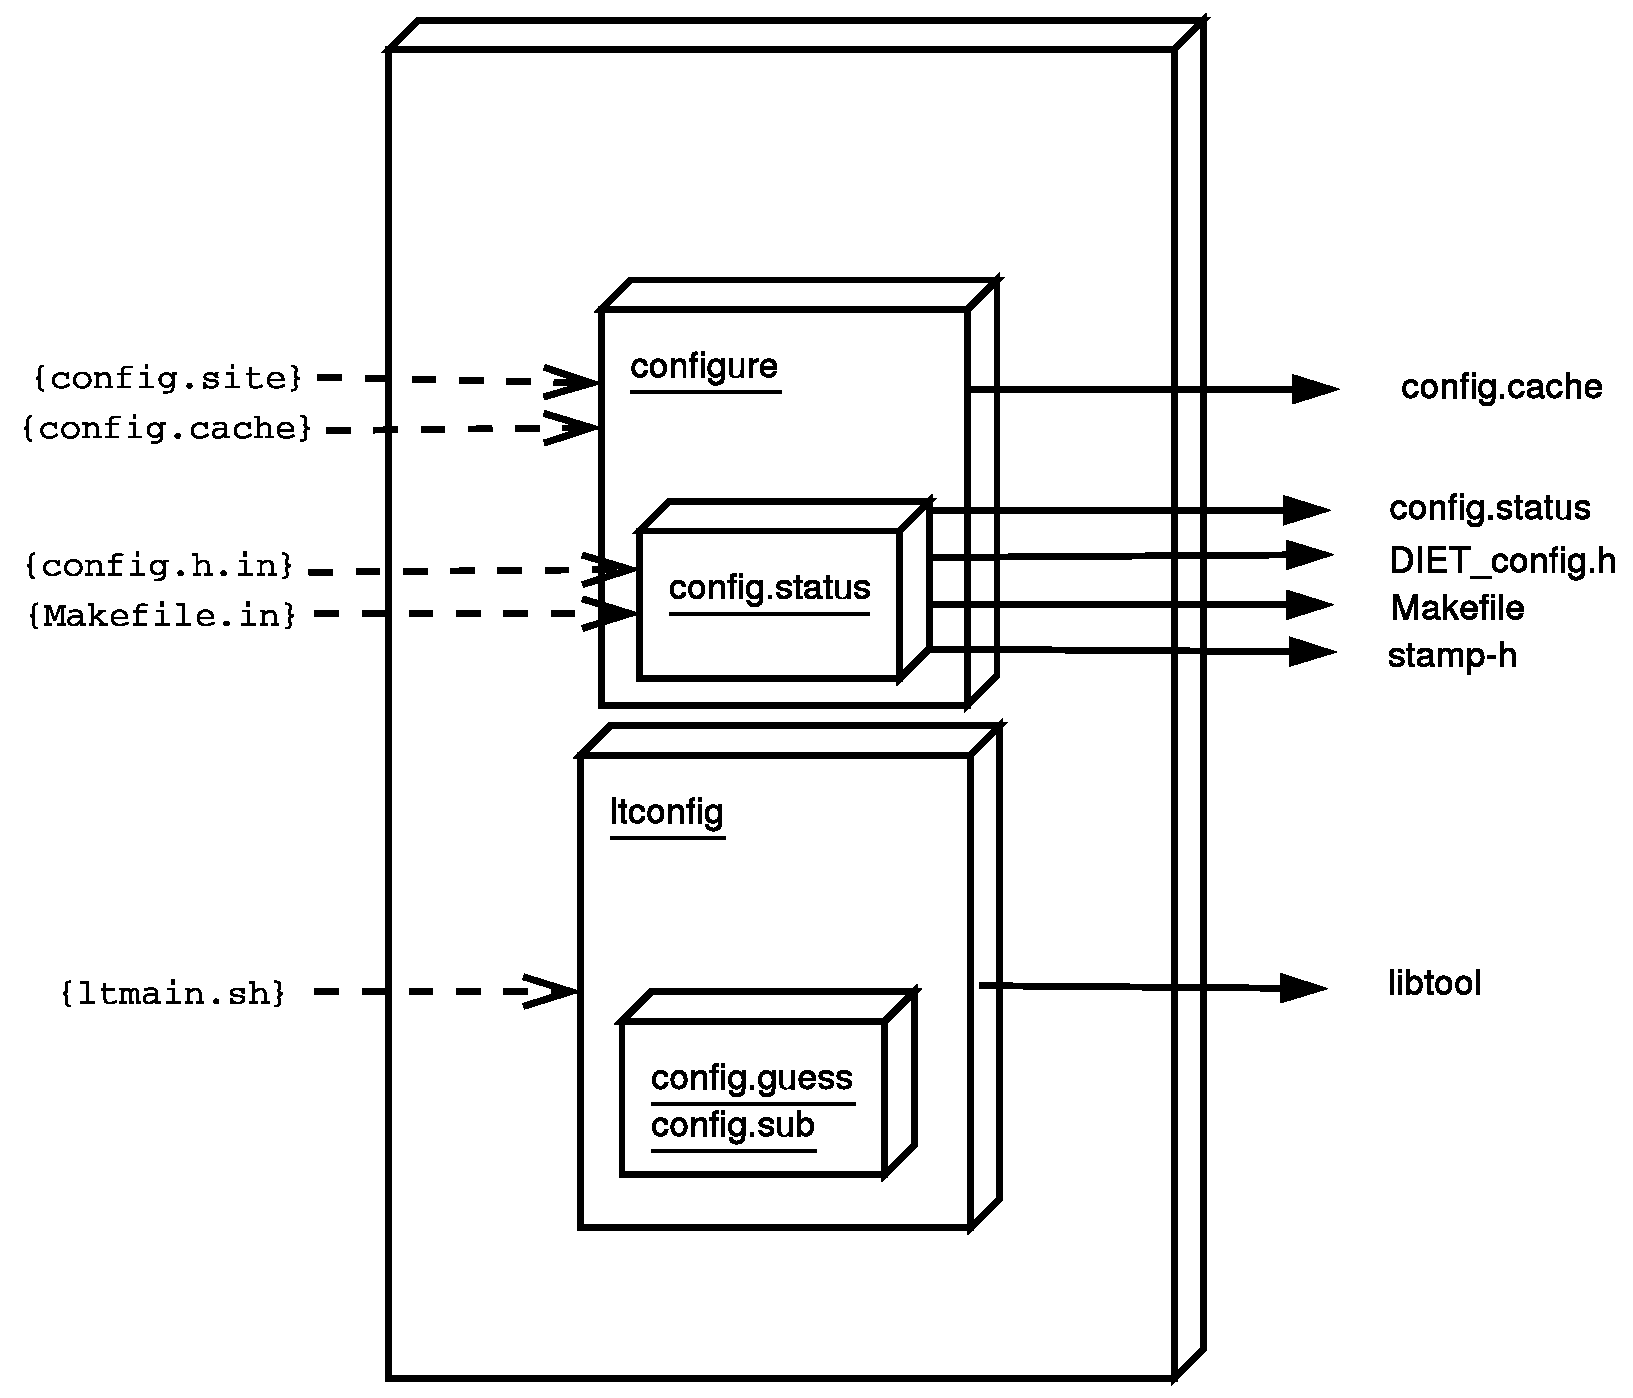
\includegraphics[scale=.35]{fig/DiagrammeConfigure.ps}
\end{center}

\section{CORBA and asynchronism}
Datas from the book "Advanced CORBA Programming with C++""
\footnote{"Advanced CORBA Programming with C++"  from Michi Henning, Steve Vinoski} and
from omniORB\footnote{OMNIORB {\url{http://www.uk.research.att.com/omniORB/}}}
and from TAO\footnote{TAO {\url{http://www.cs.wustl.edu/~schmidt/TAO.html}}
}

